\subsection{RQ2. What are the characteristics of software vulnerability detection datasets?}

Data is important for building and evaluating ML/DL-based software vulnerability detection models~\cite{lin2019software, cheng2022path, lin2018cross, du2020cross, dam2017automatic}. The quality of datasets can be assessed by different factors such as the source of data, data size and scale, data types, and preprocessing steps performed on data. For example, inappropriate preprocessing (representation) on data may result in poor performance of DL models~\cite{ruospo2020evaluating}. In this section, we examine data used in vulnerability detection studies and conducted a comprehensive analysis of the steps of data source, data type, and data representation.

\subsubsection{RQ2.1. What are the sources of datasets?}
One of the main challenges in ML/DL-based software vulnerability detection is the insufficient amount of data available for training operations~\cite{chen2020machine, lin2018cross}. Consequently, there exists a gap in research on how to obtain sufficient datasets to facilitate the training of ML/DL models for software security vulnerability detection. To this end, we analyze the sources of datasets in the studied 67 primary studies. Our analysis reveals that datasets for this purpose can be broadly classified into three categories, i.e.,  \textit{Benchmark}, \textit{Collected}, and \textit{Hybrid} sources. \textit{Benchmark} contains standardized datasets used to evaluate the performance of vulnerability detection methods and techniques~\cite{sabetta2018practical, dam2018automatic, dam2017automatic, wang2016automatically, jeon2021autovas, tian2020bvdetector, liu2020cd, yamaguchi2013chucky, liu2021combining, phan2017convolutional, nguyen2020deep, hoang2019deepjit, kronjee2018discovering, zeng2021gcn2defect, yan2021han, 3429444, 8594942, 3327890}. 

% \song{how the benchmark datasets were created? are the vulerabilities different from the collected?} 
Benchmark datasets for software vulnerability detection are often built from three main sources. The first source of data is collecting code snippets from open sources. This can include open-source software projects~\cite{jimenez2016empirical}, public vulnerability databases~\cite{black2017sard}, and bug repositories~\cite{bugzilla2021bugzilla}. The goal is to gather a diverse set of programs or code snippets that represent different application domains, programming languages, and vulnerability types. From the collected data, specific programs or code snippets are selected to be included in the benchmark dataset. The selection process considers factors such as program complexity, vulnerability diversity, and code quality. The aim is to create a dataset that covers a wide range of vulnerabilities and represents real-world scenarios. In some cases, benchmark datasets may include automatically generated synthetic programs~\cite{booth2013national}. These programs are typically created using code generation techniques and follow certain patterns or templates. Synthetic generation allows for the creation of large-scale datasets and can help cover a broader range of vulnerabilities systematically. Alongside synthetic programs, benchmark datasets often include real-world software applications or code snippets written by hand. These manually created cases ensure that the dataset contains realistic vulnerabilities that reflect actual coding practices. Manual creation involves identifying vulnerable points in the code, introducing appropriate weaknesses, and maintaining a balance between code quality and realism.

\textit{Collected} datasets are gathered from publicly available projects hosted on repository websites such as Github or Stack Overflow~\cite{chen2020machine, zhou2017automated, liu2019deepbalance, pradel2018deepbugs, cheng2021deepwukong, zhou2019devign}. Also, some studies use the combination of different sources for vulnerability detection to increase the external validity of their findings~\cite{chen2020machine, zhou2017automated, russell2018automated, wang2020combining, le2021deepcva, hin2022linevd, li2021vulnerability}, which refers to \textit{Hybrid} source in this work.

The distribution of dataset sources in the primary studies is illustrated in figure~\ref{fig:sources}. As we can see, 65.7\% of primary studies have utilized \textit{Benchmark} datasets for software vulnerability detection. 
The rationale behind this trend is that benchmark datasets are readily accessible to all researchers and can facilitate the reproducibility of prior studies. 
Researchers often used \textit{Collected} datasets in evaluating the proposed ML or DL-based security vulnerability detection models. According to our observation, 25.4\% of studies build vulnerability detection models using collected datasets.  There are a couple of reasons, first of all, open-source repositories like GitHub contain a vast amount of real-world code written by developers from diverse backgrounds. This data reflects the real-world coding practices, patterns, and vulnerabilities present in software projects. By analyzing such data, researchers can gain insights into the prevalent types of vulnerabilities and their occurrence frequencies in real-world software. Second, open-source repositories offer the opportunity to identify new vulnerabilities that may not be present in benchmark datasets. By analyzing diverse codebases, researchers can uncover previously unknown vulnerabilities or variations of known vulnerabilities, which helps in advancing the state-of-the-art in vulnerability detection and expanding the knowledge base of software security.
\begin{figure}[t!]
\centering
\begin{tikzpicture}[scale=0.5]
\pie{65.7/Benchmark,
    25.4/Collected,
    9/Hybrid}
\end{tikzpicture}
\caption{The source of the datasets used in primary study papers.}
\label{fig:sources}
\end{figure}

% \jie{i think it is not because the public dataset is not available, since when it is being published, it is already available. Maybe it is because the researchers have other requirements or some other reasons} \nima{done}
The third major source of data is \textit{Hybrid} accounting for 9\% of primary studies which is the combination of different sources. Researchers often use hybrid sources for software vulnerability detection to address some of the limitations of individual data sources and to obtain more diverse and comprehensive datasets. For example, researchers may combine data from benchmark datasets with data from other sources such as Github, open-source projects, or data from commercial companies to create a hybrid dataset that is more representative of real-world scenarios. By doing so, they can improve the generalizability of their models and increase their chances of detecting a wider range of vulnerabilities. 

% \jie{not clear what is the relation between the prior sentence and the follow-up one? For the "gather datasets", do they belong to the collected category? or constructed category? Or personally i think the collected and constructed are a little difficult to distingushed them.} \nima{I removed the figure as it was confusing. I keep the source, then I discuss the details in Table 5.}

% \song{Give some connection here, what's the relationship between the above three types and Table 5?} \nima{The next line is the connection between previous paragraphs and the table.}

Table \ref{tab:benchdetail} shows the detailed distribution of benchmark data used in the primary studies. As it is observable, \textit{NVD} and \textit{SARD} is the most widely used source of data in the \textit{Benchmark} category. This is because SARD and NVD are publicly available benchmark sources to which researchers have unrestricted access. They give a lot of vulnerability data, allowing researchers to get a broad variety of vulnerabilities for their experiments and analyses. The availability of these materials promotes repeatability and collaboration among researchers in software vulnerability detection. Overall, there are 35 unique primary studies that use benchmark datasets from different sources. 

Table \ref{tab:collectdetail} shows the detailed distribution of the \textit{Collected} source of data. As shown, \textit{Github} is the most popular source of data for software vulnerability detection, accounting for 14 primary studies. %It is a popular platform for hosting open-source software projects, it contains a vast amount of code that can be analyzed for potential vulnerabilities. 
Researchers can collect datasets from Github by crawling the platform and extracting relevant code repositories or by using Github's API to access data programmatically. One advantage of using GitHub as a source of data is that it provides access to real-world code written by developers, which can be used to train and test vulnerability detection models. This data can be particularly useful for detecting new and emerging vulnerabilities that may not be covered by benchmark datasets. Jira, CVE, and Bugzilla come after with 2 primary studies for each. Overall, there are 17 unique primary studies that use collected sources of data for software vulnerability detection. 

% \song{benchmark SVs are not written by developers??} \nima{Benchmark SVs are widely used by the community and accepted as benchmark data that everybody can use. The collected data are more specific, let say we collect data for TensorFlow for a particular SV task. Then we need to rely on collecting data from open sources. If we have specific requirements, then we need to use open-source data. We need to collect data.}

% \jie{Find it weired to mention Java and C/C++ projects, since the github source of data can also be java or c/c++ projects. This categorization is weired. } \nima{updated}


% Java and C/C++ projects are also used for software vulnerability detection as stand alone projects accounting for 10.4\% and 9.0\% of studies. This is because they offer some unique advantages compared to using benchmarks like SARD or NVD. Firstly, using standalone projects allows researchers and developers to focus specifically on the software codebase they are interested in. This can be particularly useful when working on proprietary software or in cases where benchmarks may not accurately reflect the characteristics of the codebase in question. Secondly, standalone projects often provide more detailed information about the software codebase, such as its architecture, design patterns, and dependencies. This can help researchers and developers to identify vulnerabilities that may be unique to the codebase, or to identify areas of the code that may require additional attention. The remaining 4.5\% that emerge seldom and do not belong to any group are classified as \textit{Others}. 




% \begin{table}[H]
% \caption{Distribution of combination sources for collected datasets.}
% \begin{tabular}{llcl}
% \toprule
% No & Source   & \# Studies & Description                                   & References\\
% \midrule
% 1  & Github   & 17         & A free and widely used version control system & \\
% 2  & NVD      & 15        & U.s vulnerability management system           & \\
% 3  & SARD     & 15         & A repository for security assurance tools     & \\
% 4  & Jira     & 2         & Issue tracking system                         & \\
% 5  & Bugzilla & 2         & Web-based bug tracking and testing tool       & \\
% 6  & NIST SATE & 2 & A repository of security flaws for static analysis tools & \\
% 7  & Debian   & 1         & Free and open-source Linux  distribution     & \\
% \hline
%   - & \textbf{SUM}   & \textbf{16}         & -     \\
% \bottomrule
% \end{tabular}
% \end{table}

\begin{table}[t]
\caption{Detailed distribution of benchmark sources.}
\begin{tabular}{llcp{0.55\linewidth}}
\toprule
No & Source    & \# Studies & References \\
\midrule
1  & SARD    & 17  &  \cite{jeon2021autovas,
 tian2020bvdetector,
 liu2020cd,
 wang2020combining,
 cheng2021deepwukong,
 zou2019mu,
 cao2022mvd,
 ziems2021security,
 lin2019software,
 li2021sysevr,
 filus2020random,
 li2021vuldeelocator,
 zou2019mu,
 li2021vulnerability,
 duan2019vulsniper,
 zheng2021vulspg,
 yang2022source}  \\
2  & NVD    & 13  &  \cite{jeon2021autovas,
 liu2020cd,
 wang2020combining,
 le2021deepcva,
 kronjee2018discovering,
 hin2022linevd,
 zou2019mu,
 cao2022mvd,
 li2021sysevr,
 filus2020random,
 li2021vuldeelocator,
 zou2019mu,
 zheng2021vulspg}  \\
3  & ESC and VSC & 3  &  \cite{liu2021combining, zhuang2020smart, liu2021smart}  \\
4  & SmartBugs Wild & 3  &  \cite{wu2021peculiar, nguyen2022mando, nguyen2022mando2}  \\
5  & Juliet test suit & 3  &  \cite{yan2021han, li2021vulnerability, ding2022velvet}  \\
6  & SmartBugs & 2 &  \cite{nguyen2022mando, nguyen2022mando2}  \\
7  & PROMISE    & 2 &  \cite{wang2016automatically, zeng2021gcn2defect}  \\
8  & D2A        & 2   & \cite{cheng2022path, ding2022velvet} \\
9  & NDSS    & 2  &  \cite{le2018maximal, nguyen2020deep}  \\ 
10  & NIST    & 1  &  \cite{3327890}  \\
11  & OWASP    & 1  &  \cite{3327890}  \\
12 & SAMATE    & 1      &  \cite{kronjee2018discovering}  \\
13  & Mozilla Firefox projects    & 1  &  \cite{Vuldiggerpaper}  \\
14  & ICLR2019  & 1  &  \cite{Vuldiggerpaper}  \\
15  & FQ  & 1  &  \cite{cheng2022path}  \\
16  & Bugs Wild Dataset  & 1  &  \cite{zhang2022reentrancy}  \\
17 & Others    & 1  &  \cite{nguyen2020deep}  \\
\hline
  - & \textbf{SUM}   & \textbf{53 (35)} & - \\
\bottomrule
\end{tabular}
\label{tab:benchdetail}
\end{table}

\begin{table}[t!]
\caption{Detailed distribution of Collected sources.}
\begin{tabular}{llcc}
\toprule
No & Source    &  \# Studies & References \\
\midrule
1  & Github    & 14  &  \cite{chen2020machine, zhou2017automated, liu2019deepbalance, pradel2018deepbugs, cheng2021deepwukong, zhou2019devign, pascarella2019fine, dinella2020hoppity, 3360588, fu2022linevul, chen2021neural, perl2015vccfinder, riom2021revisiting, ni2022best}  \\
2 & Jira & 2 & \cite{chen2020machine, zhou2017automated}  \\
3 & CVE & 2 & \cite{chen2020machine, zou2022mvulpreter} \\
4 & Bugzilla & 2 & \cite{chen2020machine, zhou2017automated} \\
6 & Others & 2& \cite{huang2021hunting, hoang2019deepjit} \\
\hline
  - & \textbf{SUM}   & \textbf{22 (17)} & - \\
\bottomrule
\end{tabular}
\label{tab:collectdetail}
\end{table}



\subsubsection{RQ2.2. What are the types of software vulnerability detection datasets used in prior studies?}

When it comes to detecting software vulnerabilities, datasets can have varying data types, e.g., existing software vulnerability detection models can find vulnerabilities in source code or commits. It is crucial to carefully examine the data types, as they require different preprocessing techniques and must be represented differently when using ML/DL models. Additionally, distinct data types necessitate different architectural approaches for ML/DL models. This section provides an overview of the various data types and their distributions. We classified the data types of employed datasets into three broad categories, i.e., \textit{code-based}, \textit{repository-based}, and \textit{hybrid}.

Figure \ref{fig:datasetsDist} shows the distribution of the data types in primary studies. We can observe that the majority of primary studies (70.1\%) primarily focus on analyzing the source code for software vulnerability detection. This indicates the significance of code-level analysis in identifying vulnerabilities. The utilization of repository-level data, such as commit history and change logs, is also prominent, representing a substantial portion (25.4\%) of primary studies. This suggests that repository-level information is considered valuable in vulnerability detection. Additionally, a smaller portion (4.5\%) of the studies adopt a hybrid approach, combining both code-level analysis and repository-level information. These techniques leverage the strengths of both data sources to improve the accuracy and effectiveness of vulnerability detection.

\begin{figure}[t!]
  \centering
\begin{tikzpicture}[scale=0.6]
\pie{70.1/Code,
    25.4/Repository,
    4.5/Hybrid}
\end{tikzpicture}
  \caption{The type of datasets in primary studies.}
  \label{fig:datasetsDist}
\end{figure}%

\begin{table}[t!]
\caption{Data types of datasets involved in primary studies.}
\scalebox{0.9}{
\begin{tabular}{lp{0.3\linewidth}llp{0.35\linewidth}}
\toprule
Category & Data Type             & \#Studies & Total & References\\
\midrule
\multirow{1}{*}{Code-based}                & Source code             & 42 & \multirow{1}{*}{47} & \cite{dam2018automatic,
dam2017automatic,
shippey2019automatically,
wang2016automatically,
jeon2021autovas,
tian2020bvdetector,
liu2020cd,
yamaguchi2013chucky,
liu2021combining,
kronjee2018discovering,
3172102,
zeng2021gcn2defect,
3429444,
8594942,
3327890,
zou2019mu,
cao2022mvd,
ghaffarian2021neural,
wu2021peculiar,
lin2017poster,
scandariato2014predicting,
ziems2021security,
zhuang2020smart,
li2017software,
lin2019software,
li2021sysevr,
filus2020random,
li2021vuldeelocator,
li2018vuldeepecker,
li2021vulnerability,
yamaguchi2011vulnerability,
duan2019vulsniper,
zheng2021vulspg,
zhuang2022just,
cheng2022path,
liu2021smart,
ding2022velvet,
zhang2022reentrancy,
yang2022source,
zou2022mvulpreter,
nguyen2022mando,
nguyen2022mando2} \\
         & Binary code             & 5         &   &  \cite{phan2017convolutional,
nguyen2020deep,
yan2021han,
huang2021hunting,
le2018maximal}  \\
\hline
\multirow{1}{*}{Repository-based} & Code change             & 8  & \multirow{1}{*}{13} & \cite{liu2019deepbalance, pradel2018deepbugs, zhou2019devign, dinella2020hoppity, 3360588, hin2022linevd, fu2022linevul, chen2021neural} \\
         & Commit                & 5         &      & \cite{pascarella2019fine, perl2015vccfinder, riom2021revisiting, Vuldiggerpaper, ni2022best} \\
\hline
\multirow{1}{*}{Hybrid} & Source Code+Code change & 3  & \multirow{1}{*}{7} & \cite{wang2020combining, le2021deepcva, cheng2021deepwukong} \\
 & Commits+Code Change                & 2         &      & \cite{sabetta2018practical, hoang2019deepjit}  \\
& Commits+Bug reports                & 1         &     &   \cite{zhou2017automated} \\
& Bug report+Commits+Emails & 1         &     &   \cite{chen2020machine} \\
\bottomrule
\textbf{SUM} & - &      -    &   67(67)   &  - \\
\bottomrule
\end{tabular}}
\label{datatypesdist}
\end{table}




Table \ref{datatypesdist} elaborates the detailed data types categories used in primary studies. The table shows that 42 primary studies used code-based category and the major data type of this category is \textit{Source code} \cite{zheng2021vulspg, duan2019vulsniper, yamaguchi2011vulnerability, li2021vulnerability, zou2019mu, li2021vuldeelocator, filus2020random, li2021sysevr, lin2019software, li2017software, zhuang2020smart, ziems2021security}. 
% \textit{Binary code} 
% \jie{it seems difficult to understand what is Assembly. maybe can also say it as binary code, } \nima{done} 
\textit{Binary code} is the second major data type in code-based category \cite{phan2017convolutional, huang2021hunting, yan2021han, nguyen2020deep} accounting for 5 primary studies. %We have observed that researchers tend to use binary code language instead of source code, as they believe that binary code contains more semantic information about the input data, which ultimately improves the prediction or detection performance. 
%In the field of software engineering, software repositories are a valuable source of information for solving various tasks, particularly in software security vulnerability detection. 
Regarding the \textit{Repository} based category, 13 primary studies focused on extracting useful information and patterns by crawling different artifacts from software repositories from open source. The major artifact is \textit{Code change} accounting for 8 primary studies~\cite{chen2021neural, fu2022linevul, hin2022linevd, 3360588, dinella2020hoppity, zhou2019devign, pradel2018deepbugs, liu2019deepbalance}, and \textit{Commit} comes as the second with 5 primary studies. The last category of data types is \textit{Hybrid} where the studies used a combination of different data types for software security vulnerability detection, accounting for 7 primary studies. As can be seen, \textit{Source code+Code change} is the most dominant data type combination~\cite{wang2020combining, le2021deepcva, cheng2021deepwukong}.

% \begin{figure}[H]
%     \centering
%      {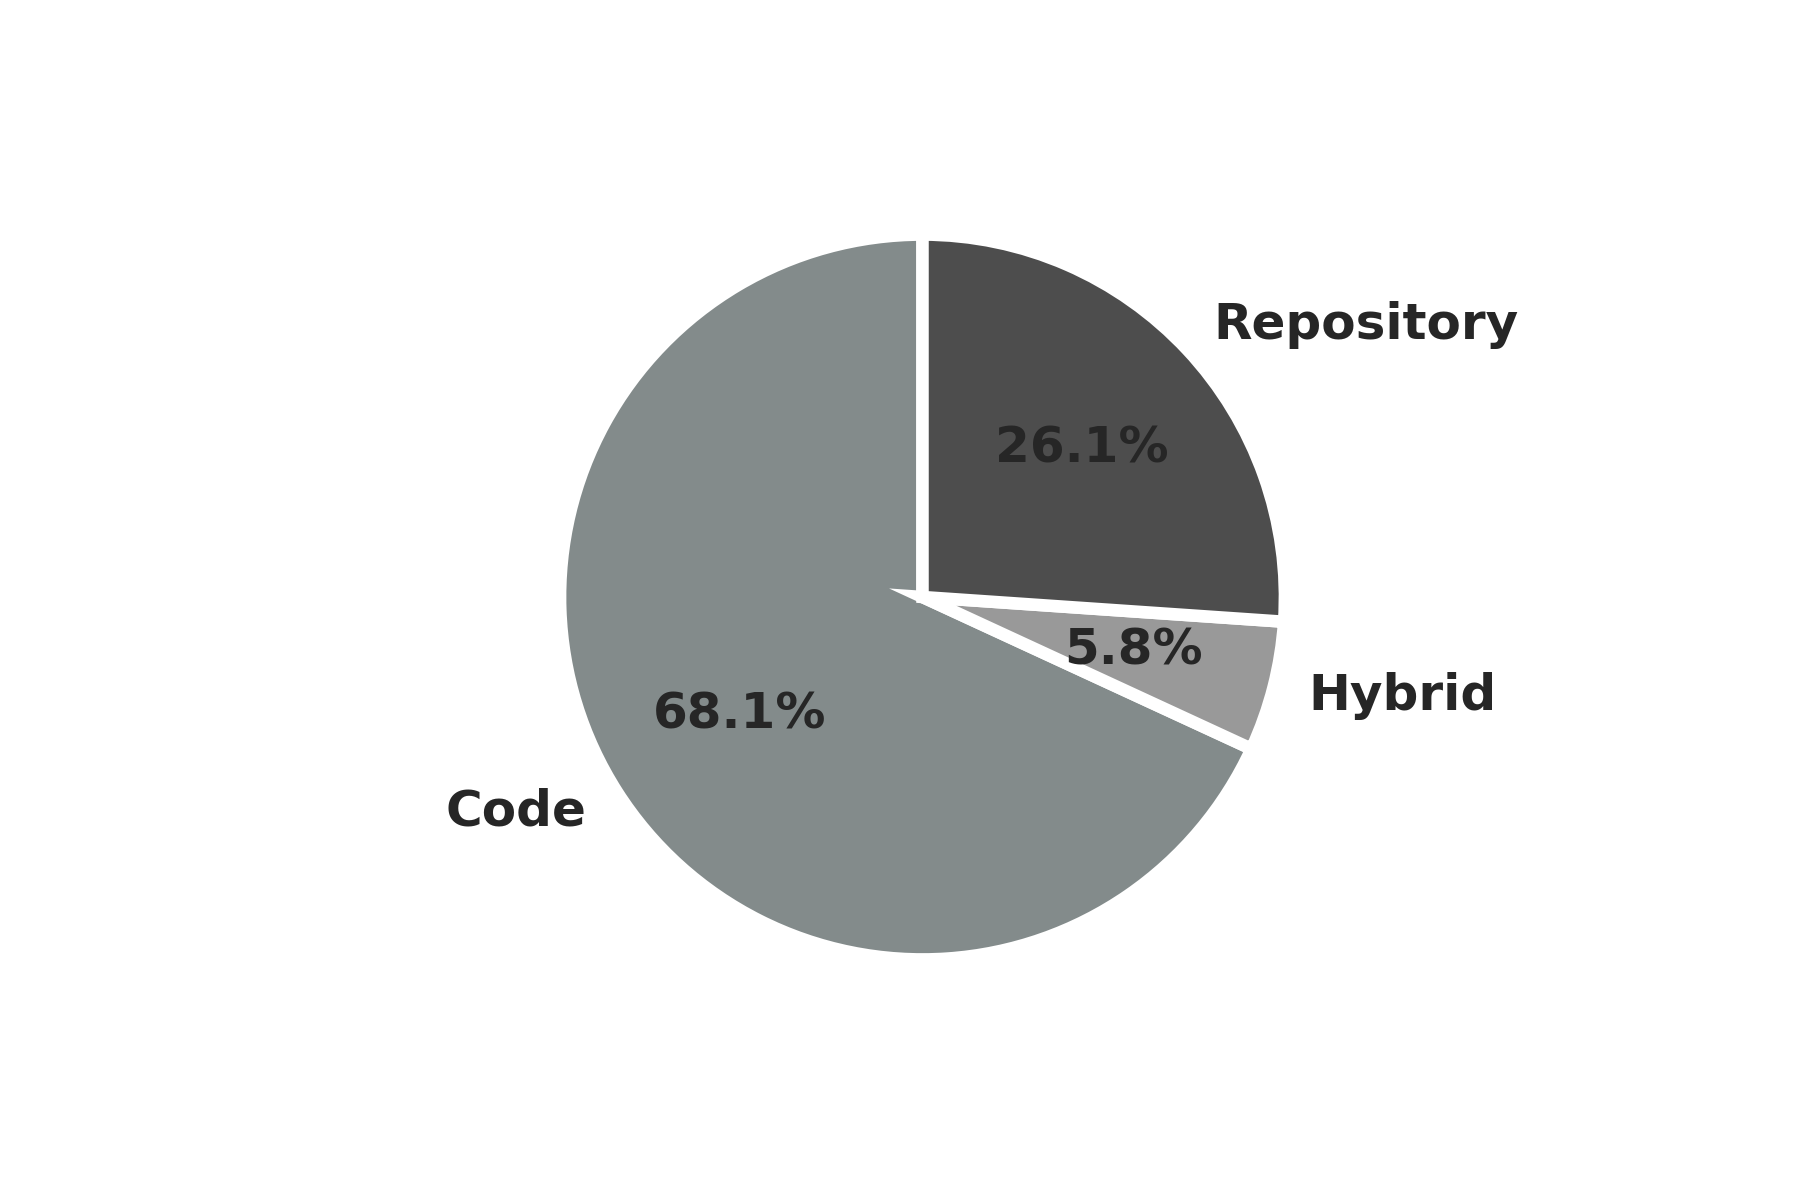
\includegraphics[width=0.8\textwidth]{Figures/RQ1/distribution_broad_type.png}}\
%      \vspace{-0.1in}
%      \caption{The type of datasets for primary studies.}
%     \label{vuldiag}
% \end{figure}




% \begin{figure}[h]
% \centering


% \newline
% \caption{Different types of datasets and representation techniques used in primary studies.\jie{I feel like the categorization cannot easily mapped to the previous discussion. for example, what is commit metrics? Only in table 8, i see the commit metrics, yet this should be merged with Hybrid, as shown in table 8. }}
% \label{fig:sources}
% \end{figure}

\subsubsection{RQ2.3. How input data are represented?}
As noted in earlier sections, research studies focused on software vulnerability detection rely on diverse sources of data and data types. This heterogeneity necessitates the use of varied representation techniques, which in turn requires different architectural approaches and design assumptions for ML/DL models.
We classified the input representation of employed datasets into five broad categories, i.e., \textit{Graph-based}, \textit{Tree-based}, \textit{Token-based}, \textit{Metric-based} and \textit{Hybrid}. Figure \ref{fig:representationDist} shows the distribution of different input representations used in primary studies. From the pie chart, we can observe that the most popular input representation is the use of \textit{Graph/Tree-based representation}, accounting for the largest slice (i.e., 38.8\% for Graph-based and 16.4\% for Tree-based). \textit{Token-based representation} follows closely, representing a substantial portion (29.9\%) of primary studies. \textit{Hybrid representation} combines multiple representations or approaches, which makes up a smaller portion (10.4\%). Finally, the use of \textit{Commit Metrics} in vulnerability detection has the smallest portion (4.5\%). In the following paragraphs, we elaborate on each category in detail. 
% \jie{it might be more accurate to say `Tree/Graph-based representation'} \nima{done}
\noindent \textbf{Graph/Tree-based representation}~\cite{jeon2021autovas, tian2020bvdetector, liu2021combining, phan2017convolutional,
cheng2021deepwukong, zhou2019devign, kronjee2018discovering, zeng2021gcn2defect,
huang2021hunting, 3360588, zou2019mu, cao2022mvd,
ghaffarian2021neural, wu2021peculiar, zhuang2020smart, li2021sysevr,
zou2019mu, duan2019vulsniper, zheng2021vulspg, cheng2022path,
liu2021smart, ding2022velvet, yang2022source, zou2022mvulpreter,
 nguyen2022mando, nguyen2022mando2}: 
allows for the detection of complex patterns and relationships between different code elements. By representing source code as a graph or tree, it becomes possible to capture not only the syntax and structure of the code but also its semantics, control flow, and data flow. There are many graph/tree-based representation techniques like Abstract Syntax Trees (AST) \cite{mao2020explainable, yamaguchi2012generalized, dinella2020hoppity, lin2017poster, lin2019software, li2021vuldeelocator} and Code Property Graph (CPG) \cite{zhou2019devign, ghaffarian2021neural, duan2019vulsniper} used to transform source code into AST and CPG representations.

\begin{figure}{t!}
  \centering
    \begin{tikzpicture}[scale=0.6]
    \pie{29.9/Token,
        38.8/Graph,
        16.4/Tree,
        10.4/Hybrid,
        4.5/Commit Metrics
        }
    \end{tikzpicture}
  \caption{Different representation used by primary studies.}
  \label{fig:representationDist}
\end{figure}%

\noindent \textbf{Token-based representation}~\cite{aivatoglou2021tree, zhou2017automated, russell2018automated, dam2018automatic, yamaguchi2013chucky, du2020cross, nguyen2020deep, liu2019deepbalance, pradel2018deepbugs, le2021deepcva, hoang2019deepjit}: treat the source code as string token sequences and then transforms source code into tokens vectors. The input data is first split into a sequence of tokens, which are then converted into numerical vectors that can be processed by machine learning algorithms. Tokenization involves breaking down a string of text or source code into smaller units, or tokens, which can then be used as the basis for further analysis. In the case of source code, tokens might include keywords, operators, variables, and other elements of the programming language syntax.


\noindent \textbf{Commit Metrics}~\cite{ni2022best, Vuldiggerpaper, pascarella2019fine}: 
leverages the metrics extracted from commits to represent code commits. Features derived from commits, such as the size of code changes, the number of modified lines, the complexity of the changes, or the programming language used, can be used as inputs to train ML/DL models. These models can then learn patterns and relationships between commit characteristics and the presence of vulnerabilities, enabling automated detection based on new commits.

\noindent \textbf{Hybrid representation}~\cite{russell2018automated, wang2020combining, le2021deepcva, cheng2021deepwukong, sabetta2018practical, hoang2019deepjit, zhou2017automated, chen2020machine}: uses a combination of different representations for software security vulnerability detection. Combining different representations of input data can lead to a more comprehensive and richer input representation of source code, which can improve the performance of vulnerability detection models in tasks such as prediction or detection. Combining different representations such as token-based representations and graph-based representations can help capture both the syntax and semantics of the code, as well as the relationships between different components of the code.



% \noindent \textbf{Feature/metric-based representation}:
% This is the traditional way of representing input data. In this paper, we do not focus on software metrics or static code attributes, rather feature-based representation chiefly means commit characteristics. 

% \jie{source code as a graph?}\nima{done}
% \jie{binary code as graph}\nima{done}
Table \ref{tbl:represenation_dist_tbl} shows the representation techniques distributed by different artifacts used by ML/DL models. It is observable that \textit{Graph/Tree-based representation} is the most dominant technique used by primary studies, accounting for 32 unique primary studies in total. These studies represent the input to ML/DL models via \textit{Source code as a graph}, \textit{Source code as a tree}, and \textit{Binary code as a graph}. \textit{Source code as a graph} is the major representation technique used by primary studies \cite{jeon2021autovas, tian2020bvdetector, liu2021combining, phan2017convolutional,
cheng2021deepwukong, zhou2019devign, kronjee2018discovering, zeng2021gcn2defect,
huang2021hunting, 3360588, zou2019mu, cao2022mvd,
ghaffarian2021neural, wu2021peculiar, zhuang2020smart, li2021sysevr,
zou2019mu, duan2019vulsniper, zheng2021vulspg, cheng2022path,
liu2021smart, ding2022velvet, yang2022source, zou2022mvulpreter,
nguyen2022mando, nguyen2022mando2} accounting for 22 studies. \textit{Source code as a tree}~\cite{dam2017automatic,
 shippey2019automatically,
 wang2016automatically,
 liu2020cd,
 wang2020combining,
 dinella2020hoppity,
 lin2017poster,
 li2017software,
 lin2019software,
 li2021vuldeelocator,
 zhuang2022just} is the second major representation technique accounting for 9 primary studies. Some researchers used \textit{Binary code as a graph}~\cite{phan2017convolutional, huang2021hunting} to build binary-level vulnerability detection models, accounting for 2 primary studies. 
% \jie{binary code?} \nima{done}
%Token-based representation is also very popular among vulnerability detection researchers \cite{dam2018automatic, yamaguchi2013chucky, hoang2019deepjit, 3429444,
%8594942, 3327890, scandariato2014predicting,
%ziems2021security, filus2020random, yamaguchi2011vulnerability, aivatoglou2021tree, zhou2017automated, du2020cross, nguyen2020deep, yan2021han, le2018maximal}. Overall, 
There are 14 primary studies that used \textit{Token-based representation}, in which 10 primary studies represented source code as a token sequence, three primary studies modeled binary code as a token, and one study represented text as token sequences~\cite{zhou2017automated}. %as a token sequence. Specifically, they used the token representation of bug reports as inputs to classical ML models.
{\textit{Hybrid} representation has 5 different types accounting for 8 primary studies. \textit{Token Sequence+Commit Metrics} is the major artifact used to enhance the input representation in software vulnerability detection, accounting for 4 primary studies. It combines information from the token sequence of the code and additional metrics derived from software commits. This approach leverages both the structural and historical aspects of the code to provide a more comprehensive representation for building vulnerability detection models.}

\textit{Commits} is the fourth least input representation used by 3 primary studies. In this representation, commit characteristics are used to build software vulnerability detection models. 

%\nima{In software vulnerability detection, the token sequence represents the sequence of tokens (e.g., keywords, identifiers, operators) present in the code snippet under analysis. It captures the syntax and structure of the code, which can provide valuable insights into potential vulnerabilities. However, relying solely on the token sequence may not capture the historical context and evolution of the codebase. To address this limitation, \textit{Token Sequence+Commit Metrics} incorporates additional information from software commits. Commits refer to the changes made to the codebase over time, typically associated with version control systems like Github. By analyzing commit information, such as the number of commits, the time interval between commits, or the number of developers involved, valuable metrics can be derived that reflect the historical characteristics of the code.}

%\song{describe how the hybird works with more detailed info of the combinations}

%Hybrid input representation is also popular in vulnerability detection studies accounting for 8 primary studies~\cite{chen2020machine, perl2015vccfinder, riom2021revisiting, ni2022best,     sabetta2018practical, fu2022linevul, li2021vulnerability,        zhang2022reentrancy}. By combining multiple representations, the vulnerability detection models can exploit the complementary strengths of each representation technique, potentially leading to improved detection accuracy. Hybrid representations enable the models to learn from different aspects of the code, leading to a more robust and effective vulnerability detection capability.

% \jie{(e.g., XXXX)}\jie{can list an example to say what kind of text}

\begin{table}[t!]
\caption{Distribution of input representations in primary studies.}
% \song{add commit metrics related papers} \nima{done}
\setlength{\tabcolsep}{3pt}
\scalebox{0.9}{
\begin{tabular}{p{0.13\linewidth}lllp{0.35\linewidth}}
\toprule
Category                                    & Artifact                      & \#Studies & Total  & References \\
\midrule
\multirow{1}{*}{Graph/Tree-based} & Source code as a graph                 & 22        & \multirow{1}{*}{32(32)}   &    \cite{jeon2021autovas,
tian2020bvdetector,
liu2021combining,
kronjee2018discovering,
zeng2021gcn2defect,
3360588,
zou2019mu,
cao2022mvd,
ghaffarian2021neural,
wu2021peculiar,
zhuang2020smart,
li2021sysevr,
li2018vuldeepecker,
duan2019vulsniper,
zheng2021vulspg,
cheng2022path,
liu2021smart,
ding2022velvet,
yang2022source,
zou2022mvulpreter,
nguyen2022mando,
nguyen2022mando2}              \\
                                            & Source code as a tree                  & 9        &    &     \cite{dam2017automatic,
shippey2019automatically,
wang2016automatically,
liu2020cd,
lin2017poster,
li2017software,
lin2019software,
li2021vuldeelocator,
zhuang2022just}             \\
                                            & Binary code as graph             & 2         &    &     \cite{phan2017convolutional,
huang2021hunting}             \\
                                            \hline
\multirow{1}{*}{Token-based} & Source code as a token                 & 10        & \multirow{1}{*}{14(14)}   & \cite{dam2018automatic,
 yamaguchi2013chucky,
 hoang2019deepjit,
 3429444,
 8594942,
 3327890,
 scandariato2014predicting,
 ziems2021security,
 filus2020random,
 yamaguchi2011vulnerability}                 \\
                                            & Binary code as a token             & 3         &    &      \cite{nguyen2020deep, yan2021han, le2018maximal}            \\
                                            & Text as a token                 & 1         &    &     \cite{zhou2017automated}             \\
\hline
\multirow{1}{*}{Hybrid} & Token Sequence+Commit Metrics & 4 & \multirow{1}{*}{8(8)}                 &      \cite{chen2020machine, perl2015vccfinder, riom2021revisiting, ni2022best}            \\
                                            & Token Sequence+Term frequency & 1         &    &      \cite{sabetta2018practical}            \\
                                            & Token Sequence+ Graph         & 1         &    &      \cite{fu2022linevul}            \\
                                            & Graph+Tree+Token Sequence     & 1         &    &      \cite{li2021vulnerability}            \\
                                            & Token+Tree     & 1         &    &      \cite{zhang2022reentrancy}            \\
\hline
\multirow{1}{*}{Commits} & Commit Metrics & 3 & \multirow{1}{*}{3}                 &      \cite{pascarella2019fine,
Vuldiggerpaper,
ni2022best}            \\
                                            \hline
\multirow{1}{*}{SUM} & - & - & \multirow{1}{*}{57(55)}                 &      \cite{pascarella2019fine,
Vuldiggerpaper,
ni2022best}            \\         
\bottomrule
\end{tabular}
}
\label{tbl:represenation_dist_tbl}
\end{table}



% \begin{figure}[H]
%     \centering
%      {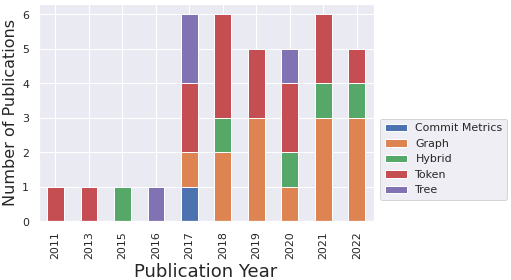
\includegraphics[width=0.6\textwidth]{Figures/RQ1/rep_by_time.png}}\
%      \vspace{-0.1in}
%      \caption{Different representation techniques distributed over time.}
%     \label{fig:rep_over_time}
% \end{figure}

\definecolor{ultrapink}{rgb}{1.0, 0.44, 1.0}
\pgfplotstableread{
Date  Commit Graph 	Hybrid 	Token 	Tree
2011 	0 	0 	0 	1 	0
2013 	0 	0 	0 	1 	0
2014	0 	0 	0 	1 	0
2015	0 	0 	1 	0 	0
2016 	0 	0 	0 	0 	1
2017 	1 	1 	0 	2 	2
2018 	0 	3 	1 	4 	1
2019 	1 	3 	0 	3 	2
2020 	0 	2 	1 	2 	1
2021 	0 	10 	2 	4 	2
2022 	1 	7 	2 	2 	2
}\testdata
\begin{figure}[t!]
\centering
\renewcommand{\arraystretch}{1}
\resizebox{0.6\columnwidth}{!}{%
    \begin{tikzpicture}[scale=0.6]
    \begin{axis}[
        ybar stacked,
    	bar width=15pt,
        ymin=0,
        ymax=20,
        xtick=data,
        legend style={at={(1.01,0.54)},anchor=west},
        reverse legend=true,
        %yticklabels from table={\testdata}{Label},
        xticklabels={ {2011}, {2013}, {2014}, {2015}, {2016}, {2017}, {2018}, {2019},
       {2020}, {2021}, {2022}},
        xticklabel style={rotate=25,anchor=east},
    ]
    \addplot + [ nodes near coords, fill=green!80]      table    [y=Commit, meta=Date, x expr=\coordindex] {\testdata};
    \addplot + [ nodes near coords, fill=cyan!80]      table    [y=Graph, meta=Date, x expr=\coordindex] {\testdata};
    \addplot + [nodes near coords, fill=blue!60]         table    [y=Hybrid, meta=Date, x expr=\coordindex] {\testdata};
    \addplot + [nodes near coords, fill=red!60]         table    [y=Token, meta=Date, x expr=\coordindex] {\testdata};
    \addplot + [nodes near coords, fill=ultrapink!60] table    [y=Tree, meta=Date, x expr=\coordindex] {\testdata};
\legend{Commits,
Graph,
Hybrid,
Token,
Tree
}
\end{axis}
\end{tikzpicture}}
\caption{Distribution of data type representations in software vulnerability detection studies over time.}
\label{typeDist}
\end{figure}



Figure \ref{typeDist} shows the distribution of data type representation in software vulnerability detection studies over time. As shown in the figure, \textit{Graph-based} representation shows a substantial presence compared to other input representation techniques. There are a couple of reasons for this trend. First, graphs provide a natural and intuitive way to represent the structural relationships within the source code. By modeling the code as a graph, the relationships between functions, classes, methods, and variables can be captured effectively. This allows vulnerability detection algorithms to analyze the code at a higher level of abstraction and capture complex dependencies and interactions between code elements. Second, graph-based representations enable a better understanding of the context in which vulnerabilities may exist. By considering the surrounding code structure and dependencies, graph-based approaches can capture the flow of information and identify potential paths that can lead to vulnerabilities. This contextual understanding helps in identifying code patterns, control flow paths, and data dependencies that may introduce security vulnerabilities. \textit{Token-based} representation has also gained popularity, with a peak occurrence in 2021. This is because it provides a fine-grained representation of the code. It simplifies the code analysis process by reducing the complexity of the code to a sequence of tokens, making it easier to apply traditional natural language processing techniques or ML models. It is also easily applicable to a wide range of programming languages. While the tokens themselves may differ across languages, the concept of breaking the code into discrete units remains the same. This versatility allows vulnerability detection techniques based on token representation to be applied to different programming languages and codebases, which further increases the external validity of vulnerability detection models. However, there is a slight decline in 2022, indicating potential shifts or diversification in the selection of input representations. \textit{Hybrid} representation is gained attention since 2021, which suggests that combining different representations is favored by researchers in software vulnerability detection, potentially due to the complementary benefits provided by multiple representations.


% Compared to a graph representation, token sequence representation is often preferred over graph representation by researchers for binaries. This is because binary code is typically a linear sequence of instructions, which can be easily represented as a token sequence. Furthermore, binary code is often optimized for performance, and the instructions are designed to be executed in a specific order. Therefore, the order of the instructions in the binary code is crucial for understanding its semantics and behavior.
% \jie{in Table 7, for the hybrid, i recommend to use the data type in the first two categories, for example Jira does not appeared in the first two categories, and maybe it is better to use `bug report'? } \nima{done}

% \jie{I didnot see the analysis of figure 4, i.e., the changes of distribution with time. also the title of figure 4 is not accurate. Furthermore, why there are five categories in this figure, what is `commits'? I am afraid i didnot explicitly see this category in Sec RQ2.3. and i assume these categories should let the reviewers clearly know where they are from. } \nima{done}


% \begin{table}[H]
% \caption{The various input forms of ML/DL based models proposed in primary studies}
% \setlength{\tabcolsep}{3pt}
% \scalebox{0.9}{
% \begin{tabular}{llllp{0.35\linewidth}}
% \toprule
% Category                                    & Artifact                      & \#Studies & Total  & References \\
% \midrule
% \multirow{}{}{Graph-based} & Code as graph                 & 26        & \multirow{}{}{39}   &    \cite{jeon2021autovas, tian2020bvdetector, liu2021combining, phan2017convolutional,
% cheng2021deepwukong, zhou2019devign, kronjee2018discovering, zeng2021gcn2defect,
% huang2021hunting, 3360588, zou2019mu, cao2022mvd,
% ghaffarian2021neural, wu2021peculiar, zhuang2020smart, li2021sysevr,
% zou2019mu, duan2019vulsniper, zheng2021vulspg, cheng2022path,
% liu2021smart, ding2022velvet, yang2022source, zou2022mvulpreter,
%  nguyen2022mando, nguyen2022mando2}              \\
%                                             & Code as tree                  & 11        &    &     \cite{dam2017automatic,
%  shippey2019automatically,
%  wang2016automatically,
%  liu2020cd,
%  wang2020combining,
%  dinella2020hoppity,
%  lin2017poster,
%  li2017software,
%  lin2019software,
%  li2021vuldeelocator,
%  zhuang2022just}             \\
%                                             & Assembly as graph             & 2         &    &     \cite{phan2017convolutional, huang2021hunting}             \\
%                                             \hline
% \multirow{}{}{Token-based} & Code as token                 & 10        & \multirow{}{}{16}   & \cite{dam2018automatic, yamaguchi2013chucky, hoang2019deepjit, 3429444,
% 8594942, 3327890, scandariato2014predicting,
% ziems2021security, filus2020random, yamaguchi2011vulnerability}                 \\
%                                             & Text as token                 & 3         &    &     \cite{aivatoglou2021tree, zhou2017automated, du2020cross}             \\
%                                             & Assembly as token             & 3         &    &      \cite{nguyen2020deep, yan2021han, le2018maximal}            \\
% \hline
% \multirow{}{}{Hybrid} & Token Sequence+Commit Metrics & 4 & \multirow{}{}{8}                 &      \cite{chen2020machine, perl2015vccfinder, riom2021revisiting, ni2022best}            \\
%                                             & Token Sequence+Term frequency & 1         &    &      \cite{sabetta2018practical}            \\
%                                             & Token Sequence+ Graph         & 1         &    &      \cite{fu2022linevul}            \\
%                                             & Graph+Tree+Token Sequence     & 1         &    &      \cite{li2021vulnerability}            \\
%                                             & Token+Tree     & 1         &    &      \cite{zhang2022reentrancy}            \\
%                                             \bottomrule
% \end{tabular}
% }
% \label{tbl:represenation_dist_tbl}
% \end{table}


% \begin{figure}[H]
%     \centering
%      {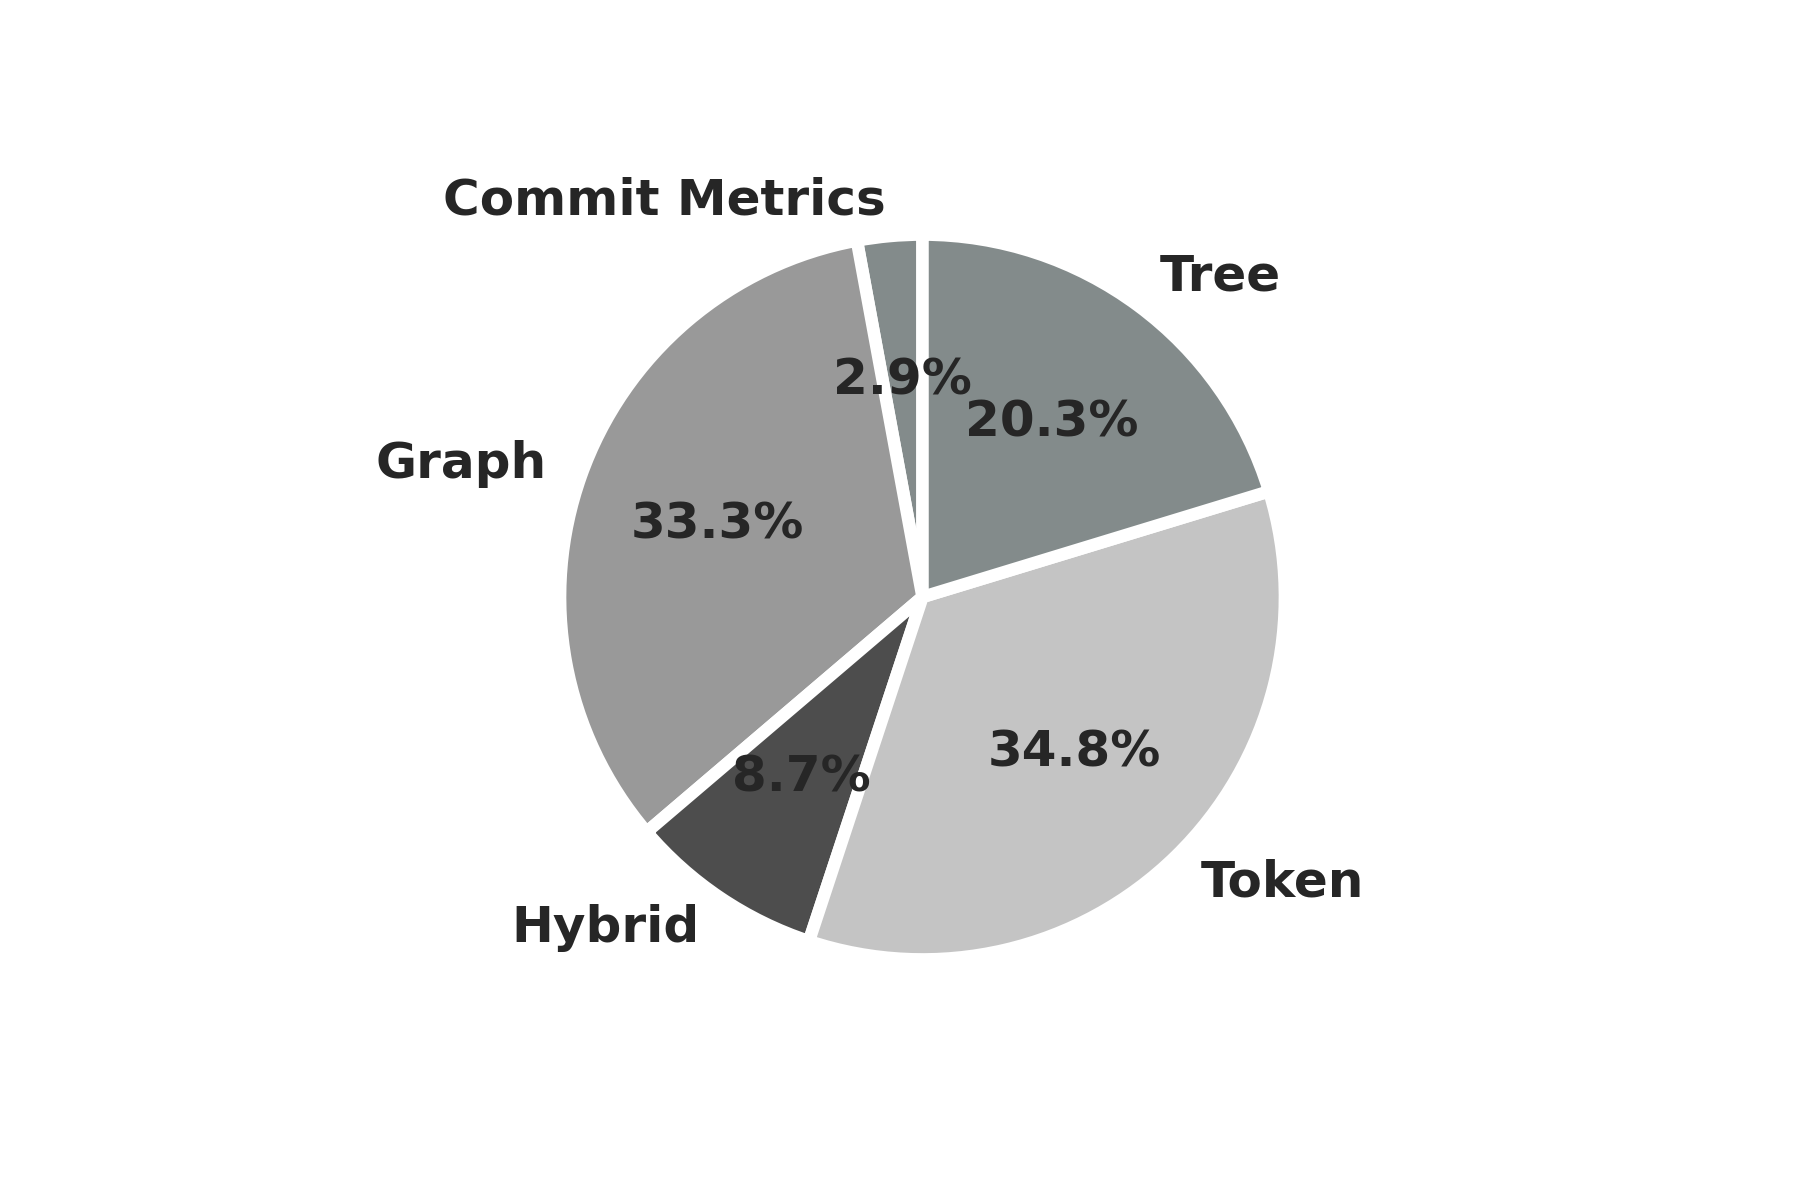
\includegraphics[width=0.8\textwidth]{Figures/RQ1/distribution_representation.png}}\
%      \vspace{-0.1in}
%      \caption{Different representation used by primary studies.}
%     \label{vuldiag}
% \end{figure}




\subsubsection{RQ2.4. How input data are embedded for feature space?}
In the previous section, we discussed various representation techniques, and in this section, we further look at embedding methods that can transform these representations into inputs that can be understood by ML/DL models. 
The representation techniques are in a human-readable format, they cannot be directly interpreted by machines. Therefore, researchers use different embedding techniques to convert these representations into a numeric format. We discuss the embedding techniques in the following paragraphs based on the distribution shown in Figure~\ref{fig:embedding_dist}. The figure illustrates the distribution of feature embedding techniques used in primary studies. The chart shows the following categories and their corresponding percentages: Word2vec (25.4\%), Graph embedding (25.4\%), Token vector embedding (11.9\%), Others (16.4\%), Hybrid (7.5\%), One hot embedding (6.0\%), Code token embedding (4.5\%), and N-gram features (3.0\%).
% \song{Give one-two sentenses to describe the categories}
% \jie{i see you list more than 3 techniques.} \nima{updated} 


\begin{figure}[t!]
    \centering
    \begin{tikzpicture}[scale=0.6]
    \pie{25.4/Word2vec,
        25.4/Graph embedding,
        11.9/Token vector embedding,
        16.4/Others,
        7.5/Hybrid,
        6.0/One hot embedding,
        4.5/Code token embedding,
        3.0/N-gram features
        }
    \end{tikzpicture}
     \vspace{-0.1in}
     \caption{Different feature embedding techniques used in primary studies.}
    \label{fig:embedding_dist}
\end{figure}

\noindent \textbf{Word2vec}~\cite{chen2020machine, sabetta2018practical, zhou2017automated, jeon2021autovas, yamaguchi2013chucky, du2020cross, lin2018cross, liu2019deepbalance, pradel2018deepbugs, zhou2019devign, yan2021han, 3360588, 3429444, 8594942, zou2019mu, scandariato2014predicting, riom2021revisiting, lin2019software, perl2015vccfinder, li2021vulnerability}: is one of the most widely-used embedding techniques for source code embedding in the examined papers, accounting for 25.4\% of primary studies. This can be because it has been shown to be effective in capturing the semantics and relationships between different code components. Word2vec can be trained on code corpus to learn embeddings for different code components, such as variables, functions, and operators. By considering the context in which these components appear, Word2vec can capture the semantic relationships between them. Furthermore, Word2vec is a computationally efficient and scalable technique, which can be trained on large code corpora. This is important for source code embedding, as the code corpus can be much larger than the text corpus typically used in natural language processing.

\noindent \textbf{Graph embedding}~\cite{liu2021combining, wang2020combining, phan2017convolutional, zeng2021gcn2defect, dinella2020hoppity, cao2022mvd, ghaffarian2021neural, wu2021peculiar, zhuang2020smart, duan2019vulsniper, zheng2021vulspg}: is another widely-used embedding technique among the primary studies, accounting for 25.4\% of primary studies, which is mostly used by graph neural networks. 
This can be because it can capture the structural relationships between different code components, such as functions, classes, and methods. In contrast to token-based representations or sequence-based representations, graph embedding can explicitly represent the connections and dependencies between different code components. In a graph-based representation, code components are represented as nodes, and the relationships between them are represented as edges. This allows for a more fine-grained representation of the code structure. 

\noindent \textbf{Token vector embedding}~ \cite{dam2018automatic, dam2017automatic, liu2020cd, wang2016automatically, hoang2019deepjit, mao2020explainable, yamaguchi2012generalized, hin2022linevd, fu2022linevul, chen2021neural, lin2017poster, yamaguchi2011vulnerability}: is also a popular technique used by primary studies accounting for 11.9\% of examined papers. In this technique, input is converted into a sequence of tokens and each token is transformed into a numeric value. Then, these values are fed into ML/DL models for further computations. 

\noindent \textbf{One hot embedding}~\cite{nguyen2020deep, hoang2019deepjit, 3327890, le2018maximal}: is a typical way for encoding categorical data, in which each category is represented by a binary vector of zeros and ones. This method can also be used to encode source code for vulnerability detection, which accounts for 6\% of studies.

\noindent \textbf{Code token embedding}~\cite{dam2018automatic, dam2017automatic, liu2020cd}: is used to represent source code tokens as dense vectors in a continuous vector space. Code token embedding captures the semantic and syntactic links between tokens by transferring them to a lower-dimensional vector space, as opposed to one hot encoding, which represents each token as a sparse binary vector.

\noindent \textbf{N-gram features}~\cite{shippey2019automatically, le2021deepcva}: is a method of expressing code snippets as fixed-length dense vectors, each vector representing an n-gram of tokens. N-grams are sequences of \verb|n| tokens, such as words or letters, that capture local context and interdependence between neighboring tokens. We observed that 3\% of primary studies use N-gram features for embedding.

% \song{put the citations for Hybrid as above} \nima{done}
\noindent \textbf{Hybrid} ~\cite{jeon2021autovas,
cheng2021deepwukong,
zhou2019devign,
3360588,
li2021vulnerability}: We find that 7.5\% of primary studies use multiple embedding techniques to convert inputs to ML/DL models. Different embedding techniques capture different aspects of the data. By combining multiple techniques, researchers can leverage the complementary information provided by each technique. For example, some embedding techniques may focus on syntax, while others may capture semantic or contextual information.

\noindent \textbf{Others}~\cite{sabetta2018practical,
kronjee2018discovering,
pascarella2019fine,
huang2021hunting,
ziems2021security,
filus2020random,
Vuldiggerpaper,
zhuang2022just,
cheng2022path,
zhang2022reentrancy,
ni2022best}: The remaining 16.4\% that emerge seldom and do not belong to any group are classified as \textit{Others}. For example, Zhang et al.~\cite{zhang2022reentrancy} customizes the graphCodeBERT~\cite{guo2020graphcodebert} to propose a graph-guided masked attention mechanism for vulnerability detection in which it captures variable dependency relationships and integrates the graph structure into the Transformer model.

% \song{Give 1-2 examples to indicate what are Others} 

\mybox{Answer to RQ2}{red!40}{gray!10}{
(1) 65.7\% of primary studies use \textit{benchmark data} for software vulnerability detection. This can be because benchmark datasets are readily accessible to all researchers and can facilitate the reproducibility of studies. 

% The second major source of data comes from the collected category where studies collect data from available repositories, accounting for 25.4\% of studies. Benchmark is the most popular source of data accounting for 38.8\% of studies. 

(2) The most common data type among the examined vulnerability detection studies is \textit{Code-based data type}, accounting for 47 studies. In this category, \textit{Source code} is the most prominent sub-type accounting for 42 studies. 

% Binary code is the second most popular sub-data type accounting for 5 studies. Software repositories are the second most data type in vulnerability detection studies. In this category, code change is the major subtype accounting for 8 studies. 

(3) \textit{Graph-based} and \textit{Token-based} input representations are the most popular input representation techniques used by primary studies accounting for 38.8\% and 29.9\% of primary studies respectively. %There is a rising trend of studies using these techniques from 2017 to 2021 indicating that these methods are attracted by many researchers.

(4) \textit{Graph embedding} and \textit{Word2vec} are the two most widely used embedding techniques used in primary studies accounting for 25.4\% of studies respectively. %The reason behind using graph embedding is the widespread usage of graph-based representation of input data.
% \jie{models? what do you want to say? In addition, do we need to summarize the embedding techniques?}
}
%\newpage
